

\chapter{Phương pháp}
\section{Phương pháp giải cổ điển}

\subsection{Thuật toán quay lui (backtracking) với bài toán xếp hậu}
Các bước thực hiện thuật toán quay lui với bài toán xếp hậu như sau:
\begin{enumerate}
    \item Khởi tạo một bàn cờ rỗng với kích thước NxN, đánh dấu tất cả các ô trên bàn cờ là chưa đặt quân hậu.
    \item Bắt đầu từ hàng đầu tiên, đặt quân hậu vào từng ô trên hàng đó. Với mỗi ô, kiểm tra xem nó có bị tấn công bởi quân hậu nào đã đặt trên bàn cờ hay không. Nếu không, đánh dấu ô đó là đã đặt quân hậu và tiếp tục đệ quy để đặt quân hậu trên hàng tiếp theo.
    \item Nếu không tìm được ô trống nào trên hàng đó để đặt quân hậu, quay trở lại hàng trước đó và thử đặt quân hậu vào ô tiếp theo trên hàng đó.
    \item Nếu đã đặt được N quân hậu trên bàn cờ, lưu trữ kết quả và thoát khỏi đệ quy.
    \item Nếu đã kiểm tra tất cả các ô trên bàn cờ nhưng không tìm được cách đặt quân hậu hợp lệ, quay trở lại và thử cách đặt quân hậu khác.
    % \item Khi đã thử tất cả các ô trên bàn cờ và lưu giữ được tất cả các lời giải, kết thúc thuật toán và trả về các lời giải đã tìm được.
\end{enumerate}

\textbf{Triển khai thuật toán:}

\begin{algorithm}[H]

\caption{Thuật toán quay lui cho bài toán xếp hậu}
\begin{algorithmic}[1]
\State $vertical = [0] * n$
\State $main\_diag =  [0] * (2 * n - 1)$
\State $anti\_diag = [0] * (2 * n - 1)$

\State
\Function{solve\_n\_queens}{n}
    \State Create an empty board of size $n \times n$
    \If{\Call{solve\_n\_queens\_util}{board, 0, n} is False}
        \State \textbf{print} "Solution does not exist"
    \EndIf
    \State \Return board
\EndFunction
\State
\Function{solve\_n\_queens\_util}{board, row, n}
    \If{row is equal to n}
        \State \Return True
    \EndIf
    \For{$col \gets 0$ \textbf{to} $n-1$}
        \If{\Call{is\_safe}{row, col, n}}
            \State Place a queen at board[row][col]
            \If{\Call{solve\_n\_queens\_util}{board, row+1, n} is True}
                \State \Return True
            \EndIf
            \State Remove the queen from board[row][col]
        \EndIf
    \EndFor
    \State \Return False
\EndFunction
\State
\Function{is\_safe}{row, col, n}
    	
        \If{vertical[col] is 1}
            \State \Return False
        \EndIf
    
  		\State $idx\_main \gets (row - col + n - 1)$
        \If{main\_diag[idx\_main] is 1}
            \State \Return False
        \EndIf

   		\State $idx\_anti \gets (row + col)$
        \If{anti\_diag[idx\_anti] is 1}
            \State \Return False
        \EndIf
    
    \State \Return True
\EndFunction
\end{algorithmic}
\end{algorithm}

Trong đó, hàm \textsc{is\_safe} kiểm tra xem một ô trên bàn cờ có thể đặt quân hậu hay không, và \textsc{solve\_n\_queens\_util} là hàm đệ quy sử dụng kỹ thuật quay lui để thử tất cả các cách đặt quân hậu trên bàn cờ. Hàm \textsc{solve\_n\_queens} tạo một bàn cờ rỗng và trả về lời giải hợp lệ.

Độ phức tạp về thời gian của thuật toán có thể được biểu thị bằng O(N!) vì trong trường hợp xấu nhất, yêu cầu phải thử tất cả các ô, tuy nhiên mỗi lần sẽ số hàng , cột giảm đi một.

\subsection{Thuật toán quy hoạch động với bài toán xếp hậu}
Thuật toán quy hoạch động cho bài toán xếp hậu được xây dựng bởi Rivin, I. và Zabih, R.\cite{dynamic programming solution} với độ phức tạp $O( f(N)*(8^N))$, với $f(N) = N^2g(N)$ là đa thức bậc thấp, $g(N)$ xuất phát từ độ phức tạp của số học số nguyên, cho bài toán xếp hậu đã chứng minh ưu việt hơn đối với cách tiếp cận quay lui đã đề cập bên trên.

Thuật toán được mô tả như sau:

Với một tập hợp các bộ dữ liệu $\langle S, i\rangle$, trong đó $S$ là tập hợp các đường (đã đặt hậu) và $i$ là một số nguyên, thể hiện một lớp tương đương của i ứng viên khả thi có tập hợp các đường đã đặt hậu là S, ta có các bước thực hiện:
\begin{enumerate}
	\item[1.] [Khởi tạo] Đặt QUEUE thành $\{\langle\emptyset, 1\rangle \}$.
	\item[2.] [Chọn ô vuông] Chọn một ô vuông chưa kiểm tra. Gọi $T$ là tập hợp bốn đường chứa ô vuông này
	\item[3.] [Vòng lặp] Với mọi tập $\langle S, i\rangle \in \text{QUEUE}$ sao cho $S \cap T = \emptyset$ thì:
	\begin{enumerate}
		\item[3.1] [Nén] Nếu $\langle S \cup T, j\rangle \in \text{QUEUE}$ đối với $j$ bất kỳ, thay $j$ bằng $i + j$.
		\item[3.2] [Tạo] Nếu không, hãy thêm $\langle S \cup T, i \rangle$ vào $\text{QUEUE}$.
	\end{enumerate}
	\item[4.] [Kết thúc] Nếu vẫn còn một ô vuông chưa được kiểm tra, hãy chuyển sang bước 2. Nếu không, hãy kết thúc.
\end{enumerate}



\section{Phương pháp giải bằng ủ lượng tử}

\subsection{Công thức bình phương cho bài toán xếp hậu}


Đầu tiên, chúng ta trình bày công thức QUBO được đề xuất bởi D-wave \cite{N Queens Dwave} sử dụng O($N^2$) biến. 
Nhưng làm cách nào để diễn đạt bài toán này dưới dạng mô hình bậc hai nhị phân(BQM)?

Để ánh xạ bài toán dưới dạng mô hình bậc hai nhị phân, chúng ta thực hiện các bước:\cite{Problem Formulation Guide} 


\textbf{Bước 1: Viết ra mục tiêu và các ràng buộc}

\textbf{Mục tiêu}: Không


\textbf{Ràng buộc}:
\begin{enumerate}
	\item Có chính xác một quân hậu trên mỗi hàng.
	\item Có chính xác một quân hậu trên mỗi cột.
	\item Có nhiều nhất một quân hậu nằm trên mỗi đường chéo chính (từ trên cùng bên trái đến dưới cùng bên phải).
	\item Có nhiều nhất một quân hậu nằm trên mỗi đường chéo phụ (từ dưới cùng bên trái đến trên cùng bên phải).
	
\end{enumerate}

\textbf{Bước 2: Chuyển đổi mục tiêu và các ràng buộc thành biểu thức toán nhị phân}

\textbf{Biến nhị phân:} Đầu tiên, chúng ta cần xác định các biến nhị phân của mình. Câu trả lời mà chúng ta đang tìm kiếm là chúng ta nên chọn ô nào. Với mỗi ô, chúng ta có thể hỏi “Chúng ta có chọn ô này để đặt hậu không?”. 

\begin{table}[H]
	\centering
	\begin{tabular}{ c c c }
		\hline
		& \textbf{Chọn ô [i,j]} & \textbf{Không chọn ô [i,j]} \\
		\hline
		\textbf{\textbf{QUBO}}     & $x_{ij} = 1$& $x_{ij} =0 $  \\
		
		\hline
	\end{tabular}
	
	
\end{table}

Khi đã xác định được các biến nhị phân, chúng ta có thể chuyển đổi mục tiêu và ràng buộc thành các biểu thức toán học.


\textbf{Mục tiêu}: Không

\textbf{Ràng buộc}:

Xét tập $Q = \{ Q_{ij} \text{ với } i, j = 1,2, \dots , n\}$, mỗi $Q_{ij}$ là một biến nhị phân với các giá trị \{0, 1\} tương ứng ô \{i, j\} không đặt và đặt quân hậu.
\begin{enumerate}
	
	\item Có chính xác một quân hậu trên mỗi hàng. 
	
	Xét tập $R = \{R_1, R_2, \dots R_n\}$, trong đó $R_u$ là tập quân hậu $Q_{ij}$ sao cho $i = u; j = 1,2, \dots , n$, ta có:
	\[
	\sum{R_u} = 1 \\ 
	\]
	
	
	\item Có chính xác một quân hậu trên mỗi cột.
	
	Xét tập $C = \{C_1, C_2, \dots C_n\}$, trong đó $C_u$ là tập quân hậu $Q_{ij}$ sao cho $i = 1,2, \dots , n; j = u$, ta có:
	\[
	\sum{C_u} = 1 \\ 
	\]
	
	\item Có nhiều nhất một quân hậu nằm trên mỗi đường chéo chính (từ trên cùng bên trái đến dưới cùng bên phải).
	
	Xét tập $D = \{D_{1-n}, D_{2-n}, \dots D_{n-1}\}$, trong đó $D_u$ là tập quân hậu $Q_{i,j}$ sao cho $i-j =u$, ta có:
	
	\[
		\sum{D_u}  \leq 1
	\]
	
	\item Có nhiều nhất một quân hậu nằm trên mỗi đường chéo phụ (từ dưới cùng bên trái đến trên cùng bên phải).
	
	Xét tập $A = \{A_2, A_3, \dots A_{2n}\}$, trong đó $A_u$ là tập quân hậu $Q_{i,j}$ sao cho $i+j =u$, ta có:
	
	\[
		\sum{A_u}  \leq 1 
	\]
	
	
	
\end{enumerate}

\textbf{Bước 3: Chuyển đổi biểu thức toán học thành mô hình bậc hai nhị phân}


Vì có chính xác một quân hậu trên mỗi hàng và cột, nên chúng ta sử dụng phiên bản tổng quát của thuật toán bao phủ chính xác \cite{Ising formulations} để xử lý các ràng buộc hàng và cột. 

Ràng buộc 1: Có chính xác một quân hậu trên mỗi hàng. (Hình \ref{fig:row-square-constraint})

\[
H_1 = \sum_{u}^{}{(1-\sum{}^{}{R_u})^2}
\]

\begin{figure}[H]
	\centering
	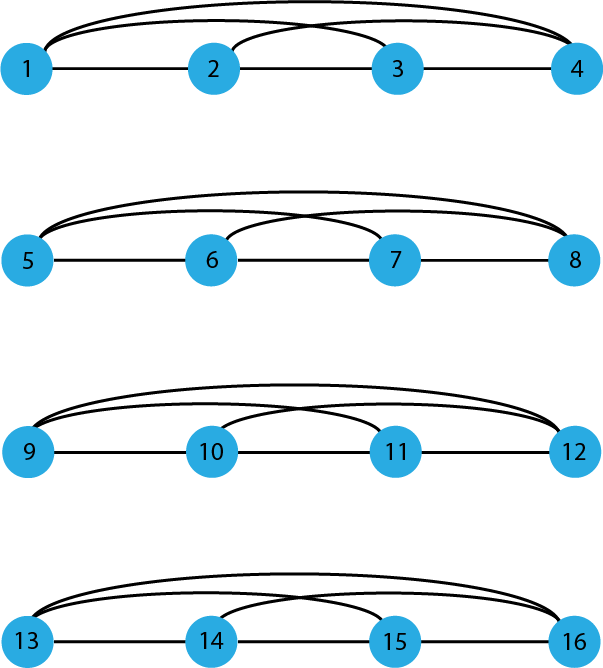
\includegraphics[width=0.5\textwidth]{images/row-square-constraint.png}
	\caption{Minh họa liên kết các ô trong ràng buộc hàng với N = 4 trong công thức bình phương}
	\label{fig:row-square-constraint}
\end{figure}


Ràng buộc 2: Có chính xác một quân hậu trên mỗi cột. (Hình \ref{fig:col-square-constraint})

\[
H_2 = \sum_{u}^{}{(1-\sum{}^{}{C_u})^2}
\]
\begin{figure}[H]
	\centering
	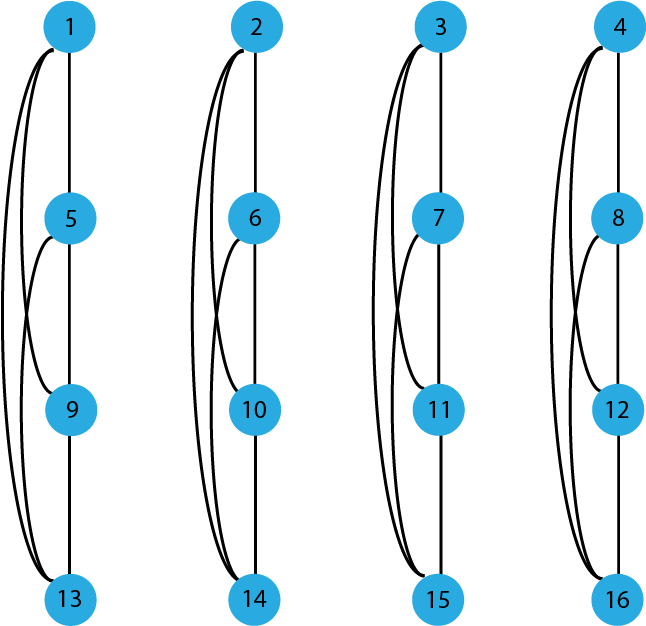
\includegraphics[width=0.5\textwidth]{images/col-square-constraint.png}
	\caption{Minh họa liên kết các ô trong ràng buộc cột với N = 4 trong công thức bình phương}
	\label{fig:col-square-constraint}
\end{figure}


Ràng buộc 3: Có nhiều nhất một quân hậu nằm trên mỗi đường chéo chính (từ trên cùng bên trái đến dưới cùng bên phải). (Hình \ref{fig:main-diag-square-constraint})

Xét $D_{ui}, D_{uj}$ tương ứng là phần tử thứ i, j của tập $D_u$, ta có:

\[
H_3 = \sum_{u}^{}{( \sum_{i<j}^{}{D_{ui}D_{uj}})}
\]

\begin{figure}[H]
	\centering
	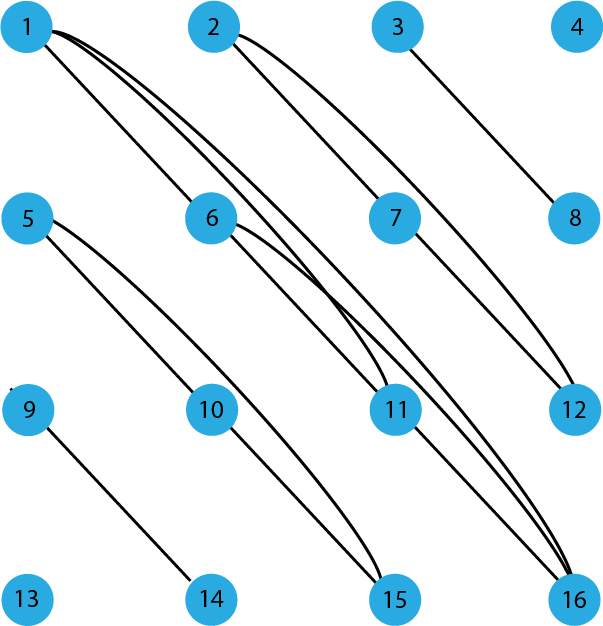
\includegraphics[width=0.5\textwidth]{images/main-diag-square-constraint.png}
	\caption{Minh họa liên kết các ô trong ràng buộc đường chéo chính với N = 4 trong công thức bình phương}
	\label{fig:main-diag-square-constraint}
\end{figure}


Ràng buộc 4: Có nhiều nhất một quân hậu nằm trên mỗi đường chéo phụ (từ dưới cùng bên trái đến trên cùng bên phải). (Hình \ref{fig:anti-diag-square-constraint})

Xét $A_{ui}, A_{uj}$ tương ứng là phần tử thứ i, j của tập $A_u$, ta có:

\[
H_4 = \sum_{u}^{}{( \sum_{i<j}^{}{A_{ui}A_{uj}})}
\]

\begin{figure}[H]
	\centering
	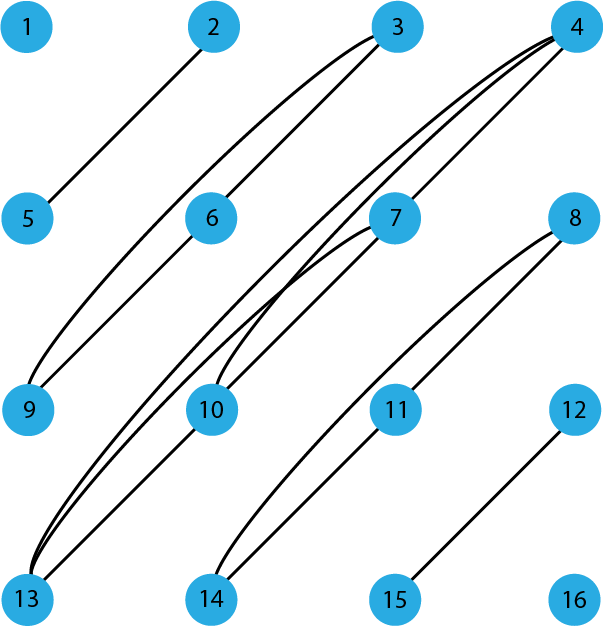
\includegraphics[width=0.5\textwidth]{images/anti_diag_square_constraint.png}
	\caption{Minh họa liên kết các ô trong ràng buộc đường chéo phụ với N = 4 trong công thức bình phương}
	\label{fig:anti-diag-square-constraint}
\end{figure}


\textbf{Bước 4: Kết hợp biểu thức}
\[
H =H_{obj}+\lambda_1 H_1+\lambda_2 H_2+\lambda_3 H_3+\lambda_4 H_4
\]

\[
	H =
	\lambda_1 \sum_{u}^{}{(1-\sum{}^{}{R_u})^2} + 
	\lambda_2 \sum_{u}^{}{(1-\sum{}^{}{C_u})^2} +
	\lambda_3 \sum_{u}^{}{( \sum_{i<j}^{}{D_{ui}D_{uj}})} +
	\lambda_4 \sum_{u}^{}{( \sum_{i<j}^{}{A_{ui}A_{uj}})}
\]

\textbf{Triển khai thuật toán:}


\begin{algorithm}[H]
    \caption{[Bình phương] Biểu thị mỗi ô trên bàn cờ bằng một tập hợp con các ID ràng buộc.}
    \begin{algorithmic}[1]
   	
    \Function{Build\_Subsets}{$n$}
	
        \State $subsets \gets \text{empty list}$
        \For{$x \text{ in range }(n)$}
            \For{$y \text{ in range }(n)$}
                \State $col \gets x$ 
                \State $row \gets y + n$ 
                \State $subset \gets \{col, row\}$
                \State $diag \gets x + y + (2*n - 1)$ 
                \State $min\_diag \gets 2*n$
                \State $max\_diag \gets 4*  n - 4$
                \If{$diag \geq min\_diag \text{ and } diag \leq max\_diag$}
                    \State $subset.add(diag)$
                \EndIf
                \State $anti\_diag \gets (n - 1 - x + y) + (4*n - 4)$ 
                
                \State $min\_anti\_diag \gets 4*n - 3$
                \State $max\_anti\_diag \gets 6*n - 7$
                \If{$anti\_diag \geq min\_anti\_diag \text{ and } anti\_diag \leq max\_anti\_diag$}
                    \State $subset.add(anti\_diag)$
                \EndIf
                \State $subsets.append(subset)$
            \EndFor
        \EndFor
        \State \Return $subsets$
    \EndFunction
    \end{algorithmic}
\end{algorithm}


Trong đó, hàm \textsc{Build\_Subsets} trả về danh sách các tập hợp con của các ràng buộc tương ứng với mọi ô trên bàn cờ. Mỗi ràng buộc được biểu thị bằng một số duy nhất (ID). Mỗi tập hợp con sẽ chứa:
\begin{enumerate}
	

	\item Chính xác một ID ràng buộc cột (0 đến n-1).
	\item Chính xác là một ID ràng buộc hàng (n đến 2*n-1).
	\item Tối đa một ID ràng buộc theo đường chéo chính (trên cùng bên trái đến dưới cùng bên phải) (4*n-3
	đến 6*n-7).
	\item Tối đa một ID ràng buộc theo đường chéo phụ (từ dưới cùng bên trái đến trên cùng bên phải) (2*n đến
	4*n-4).
\end{enumerate}
\begin{algorithm}[H]
	\caption{[Bình phương] Xây dựng mô hình bậc hai nhị phân sử dụng các tập hợp con ràng buộc}
    \begin{algorithmic}[1]
        \Function{exact\_cover\_bqm}{$problem\_set, subsets$}
            \State $bqm \gets \text{BinaryQuadraticModel}(\{\}, \{\}, 0, 'BINARY')$
            \State $cnt \gets 0$
            \For{$element$ in $problem\_set$}
                \State $bqm.offset \gets bqm.offset + 1$
                \For{$i$ in range(len($subsets$))}
                    \If{$element$ in $subsets[i]$}
                        \State $bqm.add\_variable(i, -1)$
                        \For{$j$ in range($i$)}
                            \If{$element$ in $subsets[j]$}
                                \State $bqm.add\_interaction(i, j, 2)$
                            \EndIf
                        \EndFor
                    \EndIf
                \EndFor
            \EndFor
            \State \Return $bqm$
        \EndFunction
        \State
        \Function{handle\_diag\_constraints}{$bqm, subsets, diag\_constraints$}
            \For{$constraint$ in $diag\_constraints$}
                \For{$i$ in range(len($subsets$))}
                    \If{$constraint$ in $subsets[i]$}
                        \For{$j$ in range($i$)}
                            \If{$constraint$ in $subsets[j]$}
                                \State $bqm.add\_interaction(i, j, 2)$
                            \EndIf
                        \EndFor
                    \EndIf
                \EndFor
            \EndFor
            \State \Return $bqm$
        \EndFunction
            
    \end{algorithmic}
    
\end{algorithm}

Áp dụng từ bài toán bao phủ chính xác vào ràng buộc hàng và cột, ta có hàm \textsc{exact\_cover\_bqm} trả về một mô hình bậc hai nhị phân cho một tập hợp các tập hợp con của problem\_set chứa mọi phần tử trong problem\_set đúng một lần. Hàm \textsc{handle\_diag\_constraints} cập nhật mô hình với các ràng buộc đường chéo chính (và đường chéo phụ). Nếu trùng lặp sẽ bị phạt.

\begin{algorithm}[H]
	\caption{Lấy mẫu}
	\begin{algorithmic}[1]
		
		\State $sampler \gets \text{EmbeddingComposite(DWaveSampler())}$
		\State $num\_reads \gets 1000$
		\State $sampleset \gets \text{sampler.sample(bqm, num\_reads=num\_reads)}$
		
	\end{algorithmic}
	
\end{algorithm}

Sau khi đã ánh xạ các ràng buộc vào mô hình bậc hai nhị phân, chúng ta sẽ lấy mẫu, là một tập hợp các lời giải tiềm năng chứa tập các ID ràng buộc biểu thị các ô đặt quân hậu.

\begin{algorithm}[H]
    \caption{Kiểm tra lời giải}
    \begin{algorithmic}[1]
        \Function{is\_valid\_solution}{$n, solution$}
            %\Comment{Check that solution is valid by making sure all constraints were met.}
            \State $count \gets \text{Counter}()$
            \For{$queen$ in $solution$}
                \State $count \gets count + \text{Counter}(queen)$
            \EndFor
            %\Comment{Check row/col constraints}
            \For{$i$ in range($2*n$)}
                \If{$count[i] \neq 1$}
                    \If{$i < n$}
                        \State $col \gets i$
                        \State \text{print}("Column {} has {} queens.".format($col, count[i]$))
                    \Else
                        \State $row \gets np.abs(i - (2*n - 1))$ %\Comment{Convert constraint id to row index}
                        \State \text{print}("Row {} has {} queens.".format($row, count[i]$))
                    \EndIf
                    \State \Return False
                \EndIf
            \EndFor
%            \Comment{Check diag/anti-diag constraints}
            \For{$i$ in range($2*n, 4*n - 6$)}
                \If{$count[i] > 1$}
                    \If{$i \leq 4*n - 4$}
                        \State \text{print}("Top-left to bottom-right diagonal {} has {} queens.".format($i, count[i]$))
                    \Else
                        \State \text{print}("Bottom-left to top-right diagonal {} has {} queens.".format($i, count[i]$))
                    \EndIf
                    \State \Return False
                \EndIf
            \EndFor
            \State \Return True
        \EndFunction
    \end{algorithmic}
\end{algorithm}
    
    Sau khi lấy mẫu, chúng ta sẽ kiểm tra xem lời giải có hợp lệ hay không bằng cách đảm bảo đáp ứng tất cả các ràng buộc.

\subsection{Công thức cộng dồn cho bài toán xếp hậu}

So với công thức bình phương, thì công thức cộng dồn có phần khác biệt trong cách thêm biến phụ và liên kết giữa các biến 
nên chúng ta sẽ có thay đổi ở bước 3 và bước 4.

\textbf{Bước 3: Chuyển đổi biểu thức toán học thành mô hình bậc hai nhị phân}

Ràng buộc 1: Có chính xác một quân hậu trên mỗi hàng. (Hình \ref{fig:row-square-constraint})

\[
H_1 = \sum_{u}^{}{(1-\sum{}^{}{R_u})^2}
\]


Ràng buộc 2: Có chính xác một quân hậu trên mỗi cột. (Hình \ref{fig:col-square-constraint})

\[
H_2 = \sum_{u}^{}{(1-\sum{}^{}{C_u})^2}
\]

Ràng buộc 3: Có nhiều nhất một quân hậu nằm trên mỗi đường chéo chính (từ trên cùng bên trái đến dưới cùng bên phải).


Với mỗi tập $D_u$ có $D_{ui}, D_{uj}$ tương ứng là phần tử thứ i, j của tập $D_u$, ta thêm tập các biến phụ (biến nhị phân) $S_{u}^{D} $ có $S_{ui}^{D}, S_{uj}^{D}$ tương ứng là phần tử thứ i, j của tập $S_{u}^{D}$. Ta có:

\[
H_3 = \sum_{u}^{}{\left[ (S_{u1}^{D} - D_{u1} - D_{u2})^2 + \sum_{i=2}^{}{(S_{ui}^{D} - S_{u(i-1)}^{D} - D_{u(i+1)})^2}  \right]}
\]

\begin{figure}[H]
	\centering
	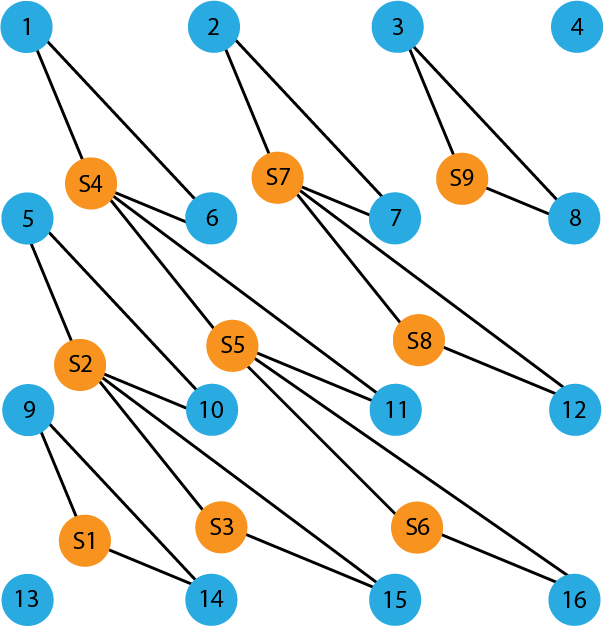
\includegraphics[width=0.5\textwidth]{images/main_diag_add_constraint.png}
	\caption{Minh họa liên kết các ô trong ràng buộc đường chéo chính với N = 4 trong công thức cộng dồn}
\end{figure}

Ràng buộc 4: Có nhiều nhất một quân hậu nằm trên mỗi đường chéo phụ (từ dưới cùng bên trái đến trên cùng bên phải).

Với mỗi tập $A_u$ có $A_{ui}, A_{uj}$ tương ứng là phần tử thứ i, j của tập $A_u$, ta thêm tập các biến phụ (biến nhị phân) $S_u^A $ có $S_{ui}^{A}, S_{uj}^{A}$ tương ứng là phần tử thứ i, j của tập $S_u^A$. Ta có:

\[
H_4 = \sum_{u}^{}{\left[ (S_{u1}^{A} - A_{u1} - A_{u2})^2 + \sum_{i=2}^{}{(S_{ui}^{A} - S_{u(i-1)}^{A} - A_{u(i+1)})^2}  \right]}
\]
\begin{figure}[H]
	\centering
	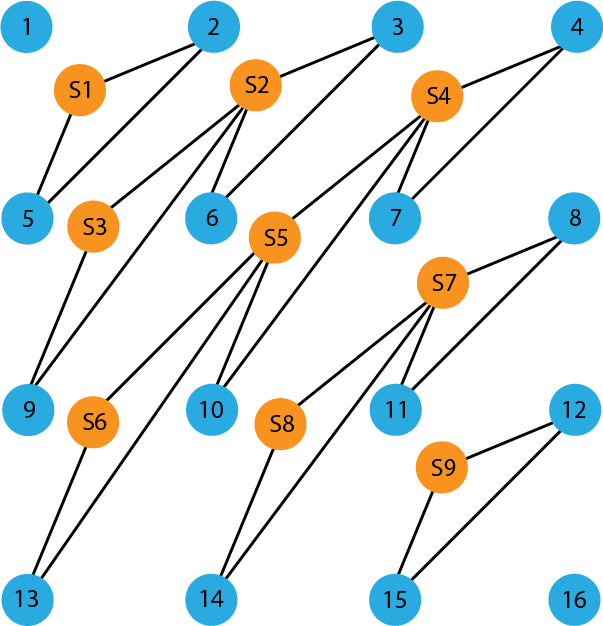
\includegraphics[width=0.5\textwidth]{images/anti_diag_add_constraint.png}
	\caption{Minh họa liên kết các ô trong ràng buộc đường chéo phụ với N = 4 trong công thức cộng dồn}
\end{figure}
\textbf{Bước 4: Kết hợp biểu thức}
\[
H =H_{obj}+\lambda_1 H_1+\lambda_2 H_2+\lambda_3 H_3+\lambda_4 H_4
\]


\begin{multline*}
	H =
	\lambda_1 \sum_{u}^{}{(1-\sum{}^{}{R_u})^2} + 
	\lambda_2 \sum_{u}^{}{(1-\sum{}^{}{C_u})^2} + \\
	\lambda_3 \sum_{u}^{}{\left[ (S_{u1}^{D} - D_{u1} - D_{u2})^2 + \sum_{i=2}^{}{(S_{ui}^{D} - S_{u(i-1)}^{D} - D_{u(i+1)})^2}  \right]} + \\
	\lambda_4 \sum_{u}^{}{\left[ (S_{u1}^{A} - A_{u1} - A_{u2})^2 + \sum_{i=2}^{}{(S_{ui}^{A} - S_{u(i-1)}^{A} - A_{u(i+1)})^2}  \right]}
 \nonumber
\end{multline*}

\textbf{Triển khai thuật toán:}

\begin{algorithm}[H]
    \caption{[Cộng dồn] Biểu thị mỗi ô trên bàn cờ bằng một tập hợp các ID}
    \begin{algorithmic}
    \For{$i$ in range($n$)}
        \State $s[i] \gets \text{dict}()$
        \For{$j$ in range($n$)}
            \State $s[i][j] \gets i \times n + j$
%            \State $varnames.append("X\{" + \text{str}(i) + "," + \text{str}(j) + "\}")$
%            \State $NumVar += 1$
        \EndFor
    \EndFor
    \State
    \State dia = \text{dict}()
    
    \For{$i$ in range($n$)}
    \For{$j$ in range($n$)}
    \If{$(i + j)$ not in dia}
    \State    dia[$i + j$] = [s[$i$][$j$]]
    \Else
    \State    dia[$i + j$].append(s[$i$][$j$])
    \EndIf
    \EndFor
    \EndFor
    
    
    \State
    \State rdia = \text{dict}()
    \For{$i$ in range($n$)}
    \For{$j$ in range($n$)}
    \If{$(i - j)$ not in rdia}
    \State rdia[$i - j$] = [s[$i$][$j$]]
    \Else
    \State rdia[$i - j$].append(s[$i$][$j$])
    \EndIf
    \EndFor
    \EndFor
    \end{algorithmic}
\end{algorithm}
    Chúng ta xây dựng một tập hợp các ID tương ứng với mọi ô trên bàn cờ theo hướng từ trái sang phải, từ trên xuống dưới, được đánh số từ 0 đến $n^2 -1$.


\begin{algorithm}[H]
    \caption{[Cộng dồn] Xây dựng mô hình bậc hai nhị phân cho ràng buộc hàng và ràng buộc cột}
    \begin{algorithmic}[1]
    \Function {exact\_cover\_bqm}{bqm, variables}:
    \State  bqm.offset += 1
    \For {i, var in enumerate(variables)}
    \State   bqm.add\_variable(var, -1)
    \For{j in range(i)}
    \State    bqm.add\_interaction(variables[j], var, 2)
       \EndFor
    \EndFor
%    \State  \Return
	
    \EndFunction
    \State
    \For{$i$ in range($n$)}
    \State  vars $\gets$ []
    \For{$j$ in range($n$)}
    \State   bqm.add\_variable(s[i][j], -1)
    \State   vars.append(s[i][j])
    \EndFor
    \State  exact\_cover\_bqm(bqm, vars)
    \State  vars $\gets$ []
    \For{$j$ in range($n$)}
    \State   vars.append(s[j][i])
    \EndFor
    \State  exact\_cover\_bqm(bqm, vars)
    \EndFor
    \end{algorithmic}
\end{algorithm}
    Chúng ta xây dựng mô hình bậc hai nhị phân cho ràng buộc hàng và cột. Và tiếp bên dưới, chúng ta cập nhật mô hình bậc hai nhị phân cho ràng buộc đường chéo chính và đường chéo phụ cho công thức cộng dồn của chúng ta.

\begin{algorithm}[H]
	\caption{[Cộng dồn] Xây dựng mô hình bậc hai nhị phân cho ràng buộc đường chéo chính và phụ}
	\begin{algorithmic}[1]
		
		\Function {add\_constraint}{bqm, S, x1, x2}:
		\State  $\lambda = 3$
		\State  bqm.add\_variable(S, $\lambda \times (1 / 2)$)
		\State  bqm.add\_variable(x1, $\lambda \times (1 / 2)$)
		\State  bqm.add\_variable(x2, $\lambda \times (1 / 2)$)
		\State  bqm.add\_interaction(S, x1, $\lambda \times (-1)$)
		\State  bqm.add\_interaction(S, x2, $\lambda \times (-1)$)
		\State  bqm.add\_interaction(x1, x2, $\lambda \times 2$)
		\EndFunction
		
		\State
		\State NumVar = $n \times n$
		\Function {dia\_constraints\_bqm}{bqm, subsetDict, type}:
		\For{k, subset\_indices in subsetDict.items()}
		\If{len(subset\_indices) $\leq$ 1}
		\State    \textbf{continue}
		\EndIf
		\State   key = type + str(k)
		\If{key not in s}
		\State    s[key] = \{\}
		\EndIf
		\State   s[key][0] = NumVar
		\State   add\_constraint(bqm, NumVar, subset\_indices[0], subset\_indices[1])
		\State   NumVar += 1
		\For{i in range(2, len(subset\_indices))}
		\State    s[key][i - 1] = NumVar
		\State    add\_constraint(bqm, NumVar, s[key][i - 2], subset\_indices[i])
		\State    NumVar += 1
		\EndFor
		\EndFor
		\EndFunction
		
		\State
		\State dia\_constraints\_bqm(bqm, dia, '+')
		\State dia\_constraints\_bqm(bqm, rdia, '-')
        
	\end{algorithmic}
\end{algorithm}

